% ==============================================================================
% DOKUMEN UTAMA (MAIN.TEX) - Dibuat Modular
% ==============================================================================

\documentclass[12pt, a4paper]{article}

% Load Preamble & Metadata
% ==============================================================================
% PREAMBLE & KONFIGURASI PACKAGES
% ==============================================================================

% Pengaturan Halaman & Margin (A4, standar 4-3-3-3 atau 3-3-3-3 cm)
\usepackage[a4paper, left=3cm, right=3cm, top=3cm, bottom=3cm]{geometry}

% Dukungan Bahasa & Karakter
\usepackage[utf8]{inputenc}
\usepackage[indonesian]{babel} % Menggunakan Bahasa Indonesia untuk penamaan (Gambar, Tabel, Bab)

% Font & Tipografi
\usepackage{times} % Menggunakan font Times New Roman (standar akademik)
\usepackage{microtype}
\usepackage{setspace}
\onehalfspacing % Spasi 1.5 (standar makalah)

% Grafik & Gambar
\usepackage{graphicx}
\usepackage{float} % Memaksa posisi gambar dengan [H]
\usepackage{caption}
\usepackage{subcaption}
\graphicspath{{figures/}} % Lokasi folder gambar

% Tabel
\usepackage{booktabs} % Garis tabel standar profesional (toprule, midrule, bottomrule)
\usepackage{multirow}
\usepackage{array}

% Matematika
\usepackage{amsmath, amssymb, amsfonts, amsthm}

% Source Code (Kodingan Robot/Data)
\usepackage{listings}
\usepackage{xcolor}

% Konfigurasi Tampilan Source Code
\definecolor{codegreen}{rgb}{0,0.6,0}
\definecolor{codegray}{rgb}{0.5,0.5,0.5}
\definecolor{codepurple}{rgb}{0.58,0,0.82}
\definecolor{backcolour}{rgb}{0.95,0.95,0.92}

\lstdefinestyle{robotstyle}{
    backgroundcolor=\color{backcolour},   
    commentstyle=\color{codegreen},
    keywordstyle=\color{blue},
    numberstyle=\tiny\color{codegray},
    stringstyle=\color{codepurple},
    basicstyle=\ttfamily\footnotesize,
    breakatwhitespace=false,         
    breaklines=true,                 
    captionpos=b,                    
    keepspaces=true,                 
    numbers=left,                    
    numbersep=5pt,                  
    showspaces=false,                
    showstringspaces=false,
    showtabs=false,                  
    tabsize=2
}
\lstset{style=robotstyle}

% Dukungan Kutipan & Bibliografi (Numeric Style standar)
\usepackage{csquotes} % Direkomendasikan untuk babel/polyglossia
\DeclareQuoteAlias{english}{indonesian}
\usepackage[backend=biber, style=numeric, sorting=none]{biblatex}
\DeclareLanguageMapping{indonesian}{english}
\addbibresource{references.bib}

% Hyperlinks (Link aktif untuk daftar isi, gambar, referensi)
\usepackage{hyperref}
\hypersetup{
    hypertexnames=false,
    colorlinks=true,
    linkcolor=black,
    filecolor=magenta,      
    urlcolor=blue,
    pdftitle={Makalah UAS ISR},
    pdfpagemode=FullScreen,
}

% Pengaturan Paragraf & Indentasi
\setlength{\parindent}{1cm}
\setlength{\parskip}{0.2cm}

% ==============================================================================
% METADATA MAKALAH UAS ISR
% ==============================================================================
% Silakan sesuaikan informasi di bawah ini dengan data kelompok Anda.

\newcommand{\JudulMakalah}{Perancangan dan Implementasi Sistem Robotika Berbasis Intelligent Systems}
\newcommand{\JudulSingkat}{Robotika Berbasis Intelligent Systems}
\newcommand{\MataKuliah}{Instrumentasi Sistem Robotika}
\newcommand{\TahunAkademik}{2026}
\newcommand{\DosenPengampu}{Dr.Eng. Dwi Joko Suroso, S.T., M.Eng.}
\newcommand{\ProgramStudi}{Departemen Teknik Nuklir dan Teknik Fisika}
\newcommand{\Fakultas}{Fakultas Teknik}
\newcommand{\Universitas}{Universitas Gadjah Mada}

% Anggota Kelompok
\newcommand{\AnggotaSatu}{Muhammad Khalis Farhan Azvi}
\newcommand{\NIMSatu}{22/493199/TK/54016}

\newcommand{\AnggotaDua}{Valen Fatli}
\newcommand{\NIMDua}{22/493755/TK/54109}

\newcommand{\AnggotaTiga}{Yasir Abdulaziz}
\newcommand{\NIMTiga}{22/497079/TK/54468}

\newcommand{\AnggotaEmpat}{Galih Salman Sadewo}
\newcommand{\NIMEmpat}{22/498121/TK/54625}

\newcommand{\AnggotaLima}{Faris Afif Ridyasmara}
\newcommand{\NIMLima}{22/502798/TK/54902}


\begin{document}

% ==============================================================================
% COVER PAGE (HALAMAN JUDUL)
% ==============================================================================
\begin{titlepage}
    \centering
    
    % Judul Makalah (Bold, All Caps, Ukuran Besar)
    {\setstretch{1.3}
    {\large \textbf{LAPORAN TUGAS AKHIR UAS}}\\[0.5cm]
    {\Large \textbf{\JudulMakalah}}\\[1.5cm]
    }
    
    % Logo Universitas (Disimpan di folder figures/)
    
\includegraphics[width=4cm]{figures/Lambang UGM-hitam.png}\\[1.5cm]
    
    % Keterangan Anggota Kelompok (Sesuai dengan permintaan UAS)
    \textbf{Disusun Oleh (Kelompok UAS):}\\[0.4cm]
    \begin{tabular}{ccc}
        \textbf{Nama} & & \textbf{NIM} \\
        \midrule
        \AnggotaSatu & --- & \NIMSatu \\
        \AnggotaDua   & --- & \NIMDua \\
        \AnggotaTiga  & --- & \NIMTiga \\
        \AnggotaEmpat & --- & \NIMEmpat \\
        \AnggotaLima  & --- & \NIMLima \\
    \end{tabular}\\[0.6cm]
    
    % Detail Institusi & Kelas
    {\large
    \textbf{Course Lecturer: \DosenPengampu}\\[1cm]
    \textbf{\MataKuliah}\\[0.3cm]
    \ProgramStudi\\[0.2cm]
    \Fakultas\\[0.2cm]
    \Universitas\\[0.2cm]
    Tahun \TahunAkademik
    }
    
\end{titlepage}

% ==============================================================================
% HALAMAN DAFTAR ISI & PENGANTAR
% ==============================================================================
\pagenumbering{roman} % Nomor halaman romawi untuk daftar isi

\newpage
\tableofcontents
\newpage
\listoffigures
\listoftables

\newpage
\pagenumbering{arabic} % Kembali ke penomoran angka standar untuk isi bab

% ==============================================================================
% KONTEN UTAMA (MODULAR SECTIONS)
% ==============================================================================
\section{Pendahuluan}
\label{sec:pendahuluan}

\subsection{Latar Belakang}
Tuliskan latar belakang topik proyek robotika atau sistem cerdas yang Anda kerjakan di sini. Latar belakang harus mencakup penjelasan mengenai permasalahan riil yang melandasi pentingnya pembuatan sistem robot ini, penelitian terdahulu yang relevan, serta solusi cerdas yang diajukan dalam proyek ini. 

Contoh pengacuan pustaka menggunakan LaTeX: Robot ini dirancang untuk mengatasi permasalahan navigasi otonom menggunakan algoritma tertentu \parencite{author2026example}.

\subsection{Rumusan Masalah}
Berdasarkan latar belakang di atas, rumusan masalah dalam penelitian/proyek ini adalah:
\begin{enumerate}
    \item Bagaimana merancang arsitektur perangkat keras dan lunak pada robot agar mampu beroperasi secara cerdas?
    \item Bagaimana performa algoritma kontrol/navigasi yang diimplementasikan pada sistem robot tersebut?
    \item Sejauh mana tingkat akurasi pembacaan sensor dalam mengenali kondisi lingkungan sekitar?
\end{enumerate}

\subsection{Tujuan Penelitian}
Tujuan dari pelaksanaan proyek UAS Intelligent Systems and Robotics ini adalah:
\begin{enumerate}
    \item Merancang dan mengimplementasikan sistem robotika terintegrasi yang mampu melakukan [tuliskan tugas spesifik robot].
    \item Menganalisis kinerja sensor dan aktuator yang digunakan pada platform robot.
    \item Menguji keandalan sistem kontrol cerdas dalam skenario lingkungan nyata.
\end{enumerate}

\subsection{Manfaat Penelitian}
Hasil dari rancang bangun sistem robotika ini diharapkan dapat memberikan manfaat sebagai berikut:
\begin{itemize}
    \item \textbf{Bagi Mahasiswa:} Meningkatkan pemahaman praktis mengenai integrasi sensor, aktuator, dan algoritma kecerdasan buatan pada sistem fisik.
    \item \textbf{Bagi Akademisi:} Menjadi referensi tambahan dalam pengembangan sistem navigasi robotika otonom skala laboratorium.
    \item \textbf{Bagi Praktisi:} Memberikan inspirasi desain sistem robotika berbiaya rendah dengan performa yang andal.
\end{itemize}

\newpage

\section{Tinjauan Pustaka}
\label{sec:tinjauan_pustaka}

Bagian ini memaparkan teori dasar yang mendukung pengerjaan proyek robotika ini. Teori-teori ini mencakup sensor yang digunakan, sistem kendali, serta algoritma kecerdasan buatan yang ditanamkan pada robot.

\subsection{Sistem Kendali Robot (Intelligent Controls)}
Sistem kontrol pada robot sering menggunakan algoritma seperti Proportional-Integral-Derivative (PID), Fuzzy Logic, atau kecerdasan buatan lainnya. Kontrol cerdas ini memungkinkan robot untuk mengambil keputusan secara dinamis berdasarkan data sensor secara real-time.

\subsection{Sensor Jarak dan Penginderaan Lingkungan}
Untuk menavigasi lingkungan, robot dilengkapi dengan sensor jarak seperti Ultrasonik (HC-SR04), LiDAR, atau kamera. Persamaan dasar perhitungan jarak pada sensor ultrasonik adalah:
\begin{equation}
    s = \frac{v \times t}{2}
    \label{eq:ultrasonic}
\end{equation}
di mana $s$ adalah jarak objek (meter), $v$ adalah kecepatan rambat suara di udara ($\approx 340$ m/s), dan $t$ adalah waktu tempuh gelombang pantul (detik).

\subsection{Platform Mikrokontroler / Single Board Computer}
Robot ini menggunakan platform mikrokontroler [tuliskan nama board, misal: Arduino Uno, ESP32, Raspberry Pi, Jetson Nano] sebagai unit pemroses utama. Unit ini bertugas membaca data input dari sensor, melakukan pemrosesan algoritma navigasi, dan memberikan sinyal kendali PWM (Pulse Width Modulation) ke driver motor.

\newpage

\section{System Design}
\label{sec:perancangan_sistem}

This chapter describes the comprehensive robotic system design architecture, which is divided into hardware configuration, computer vision subsystem, and navigation control logic.

\subsection{Hardware Architecture}
\label{subsec:hardware_architecture}

The hardware architecture of the autonomous color-tracking robot is designed as an integrated embedded robotic platform. Conceptually, this system is divided into four main functional blocks: the processing and control unit, the sensing system, the actuation mechanism, and the power distribution topology. The data flow, control signals, and power distribution among these functional blocks are represented by the high-level architecture diagram in Figure \ref{fig:diagram_hardware}.

\begin{figure}[H]
    \centering
    % Ensure the file name matches your repository
    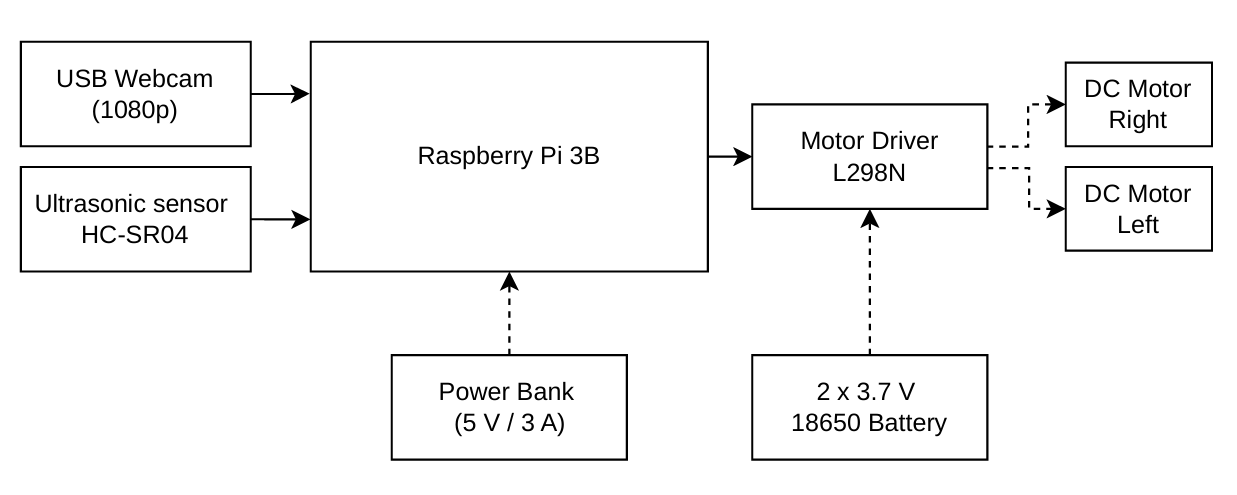
\includegraphics[width=0.8\textwidth]{block_diagram.jpg} 
    \caption{Block diagram of the hardware architecture and control signal flow.}
    \label{fig:diagram_hardware}
\end{figure}

\subsubsection{Processing and Control Unit}
The core computational and control operations of the entire system rely on a Raspberry Pi 3 Model B Single-Board Computer (SBC). The use of this SBC is essential to provide the considerable computational resources required to execute the OpenCV-based image processing algorithms and bounding-box generation without relying on external computing. The Raspberry Pi acts as the main processing and control unit that reads the continuous visual data stream, processes the navigation decision logic, and translates these calculations into Pulse Width Modulation (PWM) control signals. These signals are subsequently distributed through the General Purpose Input/Output (GPIO) pins to dictate the responses of the actuation system.

\subsubsection{Sensing System}
The robot's ability to perceive its surroundings and gather environmental information is realized through the integration of two distinct sensing technologies:
\begin{itemize}
    \item \textbf{Monocular Camera (1080p USB Webcam):} Serving as the primary visual sensor, the webcam captures light reflections from objects and converts them into RGB pixel matrices. These raw data matrices are streamed to the processing unit to be transformed into the HSV color space. This mapping is fundamental for the vision-based system, as it separates pure chromatic information (Hue) from environmental illumination intensity (Value). This enhances the robustness of the HSV-based segmentation, allowing the robot to identify the color-defined target and extract bounding boxes even under varying lighting conditions.
    \item \textbf{Ultrasonic Sensor (HC-SR04):} Operating based on the Time-of-Flight (ToF) principle of mechanical waves, this sensor emits 40 kHz ultrasonic pulses and calculates the time elapsed until the echo is received. It is implemented as a frontal distance sensor to provide direct physical distance measurements and support reactive collision-avoidance decisions. If a frontal obstacle is detected within a critical proximity, the sensor input triggers an interrupt in the main control logic to immediately halt traction, preventing physical collisions when the visual sensor is occluded or experiences response latency.
\end{itemize}

\subsubsection{Actuation and Kinematic Control}
The conversion of electrical control signals into mechanical torque is managed by a differential drive configuration, suitable for a two-wheeled mobile robot.
\begin{itemize}
    \item \textbf{L298N Motor Driver Circuit:} This module functions as a power interface bridge between the Raspberry Pi's low-voltage GPIO pins (3.3V) and the inductive load of the motors, which demands high current supply. Operating on a Dual H-Bridge circuit topology, the L298N allows dynamic voltage polarity reversal to control the direction of motion, while simultaneously switching the PWM signals from the processing unit to regulate the duty cycle (rotational speed).
    \item \textbf{Direct Current (DC) Motors:} The final motion execution relies on two DC motors coupled to the left and right wheels of the chassis. By asynchronously varying the rotational speed distribution between the two wheels, the robot can perform skid-steering to smoothly execute required motion commands, including moving forward, turning left, turning right, stopping, and performing obstacle-avoidance maneuvers.
\end{itemize}

\subsubsection{Power Distribution Topology}
The computational stability of the embedded platform heavily depends on the implemented power supply scheme. Because DC motors are inductive loads—prone to generating inrush currents upon starting and back-Electromotive Force (back-EMF)—the system employs a split power supply topology with an integrated common ground.
\begin{itemize}
    \item \textbf{Logic Power Supply:} The Raspberry Pi is exclusively powered by a closed power source (5V/3A Powerbank). Isolating this current source is crucial to maintain computational voltage stability and prevent transient voltage drops that could reset the operating system kernel when the actuators operate at maximum capacity.
    \item \textbf{Mechanical Load Power Supply:} The L298N driver circuit and the DC motors receive power from a series configuration of two 18650 Lithium-ion batteries. The 7.4V nominal voltage from this array is injected directly into the driver's input terminals. Although the power sources are physically separated, the ground terminals (GND) of the 18650 battery circuit and the Raspberry Pi's GPIO are strictly unified. This common ground ensures that all PWM control pulses share a uniform zero-equipotential reference, guaranteeing that the operational logic is translated precisely without noise interference.
\end{itemize}

\vspace{1em}
The physical implementation of these integrated hardware components on the mechanical chassis is shown in Figure \ref{fig:fisik_robot}. This concrete integration of functional blocks ultimately enables the mobile robot to acquire actual environmental parameters, execute lightweight object-detection methods, and perform precise kinematic maneuvers.

\begin{figure}[H]
    \centering
    % Ensure the file name matches your repository
    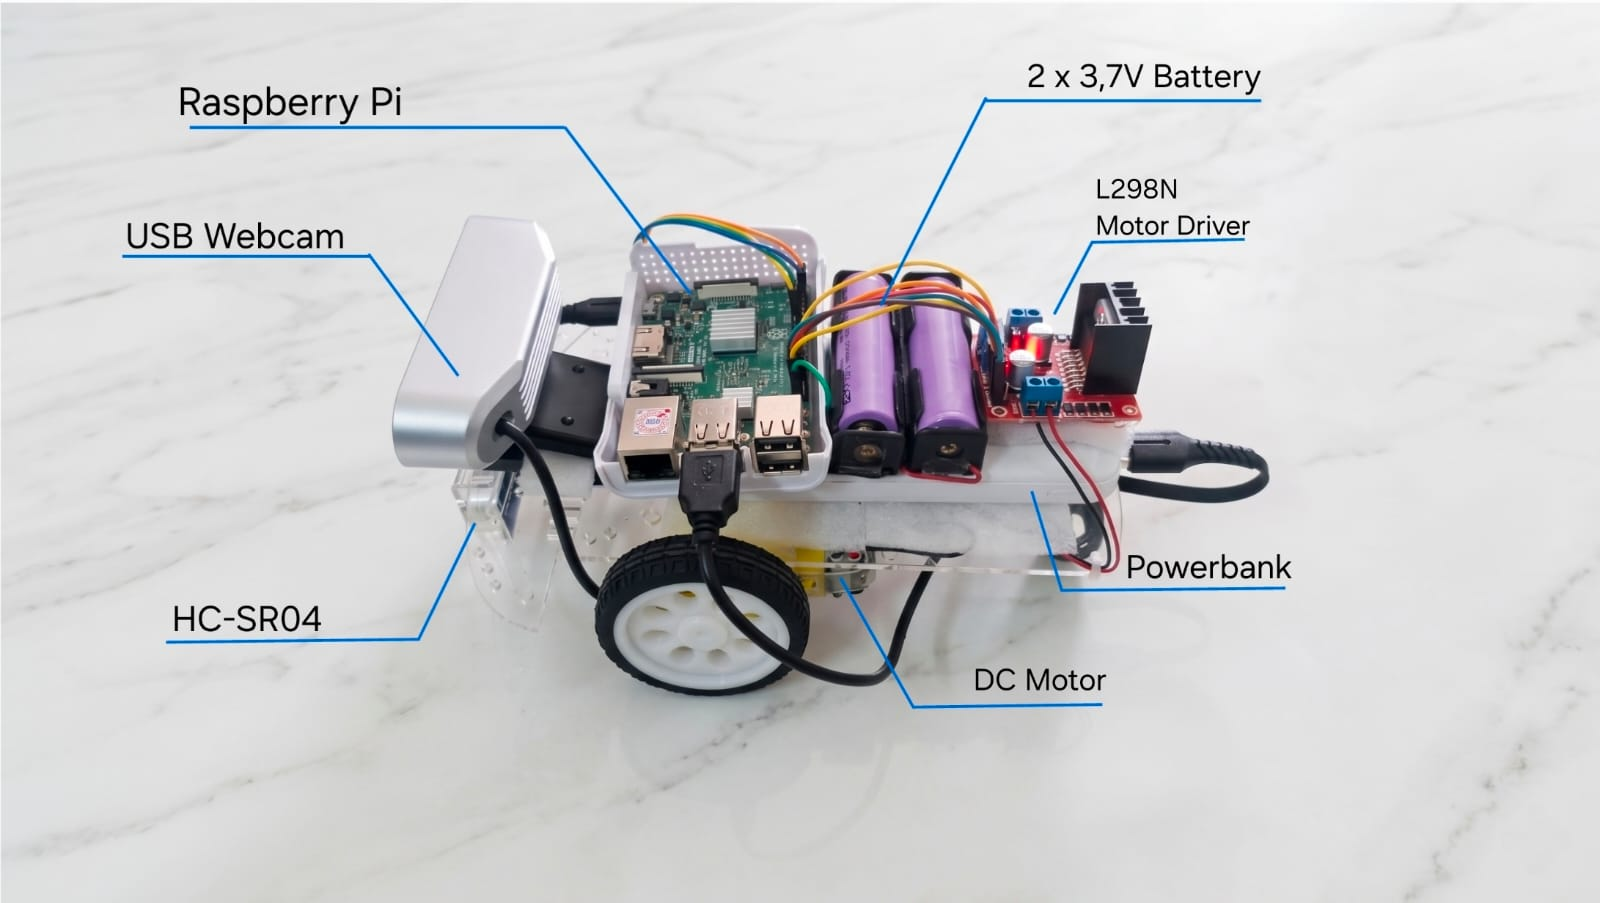
\includegraphics[width=0.7\textwidth]{gambar_robot.jpg} 
    \caption{Physical hardware implementation on the autonomous color-tracking robot chassis.}
    \label{fig:fisik_robot}
\end{figure}

\subsection{Visual System Design (Visual)}
The design of the visual subsystem focuses on the real-time processing of digital images captured by a USB Webcam. The camera is positioned at the front of the robot to capture the environmental conditions directly. The processing pipeline of this visual system is divided into four main stages: image acquisition, preprocessing and color segmentation (masking), object contour detection, and visual distance estimation.

\subsubsection{Image Acquisition and Camera Management (\textit{camera\_manager.py})}
Raw images are obtained using a USB Webcam with a native resolution of $320 \times 240$ pixels. The video capture format is set using MJPG (\textit{Motion JPEG}) compression via the V4L2 (\textit{Video for Linux 2}) driver to minimize USB bandwidth usage and the processing load on the Raspberry Pi.

To avoid bottlenecks in the execution of the main program, the camera frame reading process is isolated into a separate background thread that runs asynchronously with a sleep interval of $0.03$ seconds between frame captures. This ensures that the latest frame is always available and ready to be accessed by the image processing module at any time without blocking the main execution thread. The camera management implementation code can be seen in Listing~\ref{lst:camera_manager}.

\begin{lstlisting}[language=Python, caption={Camera Manager Module Code (camera\_manager.py)}, label={lst:camera_manager}]
import cv2
import threading
import time
import numpy as np

class CameraManager:
    def __init__(self, src=0):
        self.src = src
        # Use V4L2 backend which is much more stable on Raspberry Pi/Linux
        self.stream = cv2.VideoCapture(self.src, cv2.CAP_V4L2)
        
        # Set format to MJPG to save USB bandwidth on Raspberry Pi
        self.stream.set(cv2.CAP_PROP_FOURCC, cv2.VideoWriter_fourcc(*'MJPG'))
        self.stream.set(cv2.CAP_PROP_FRAME_WIDTH, 320)
        self.stream.set(cv2.CAP_PROP_FRAME_HEIGHT, 240)
        
        self.grabbed = False
        # Initialize with a black frame so it is not None
        self.frame = np.zeros((240, 320, 3), dtype=np.uint8)
        self.stopped = False
        
        if self.stream.isOpened():
            print(f"[CAM] Camera {self.src} detected.")
            # Capture one initial frame synchronously
            self.grabbed, self.frame = self.stream.read()
        else:
            print(f"[CAM] [ERROR] Camera {self.src} not found!")

    def start(self):
        # Run frame reading in the background thread
        threading.Thread(target=self.update, args=(), daemon=True).start()
        return self

    def update(self):
        while not self.stopped:
            if not self.stream.isOpened():
                break
            self.grabbed, self.frame = self.stream.read()
            # Small delay to not overload the CPU
            time.sleep(0.03)

    def read(self):
        return self.frame

    def stop(self):
        self.stopped = True
        self.stream.release()

    def switch_source(self, new_src):
        """Dynamically switch camera input"""
        self.stopped = True
        time.sleep(0.1)  # Give a small delay for the update thread to finish
        self.stream.release()
        
        self.src = new_src
        self.stream = cv2.VideoCapture(self.src, cv2.CAP_V4L2)
        self.stream.set(cv2.CAP_PROP_FOURCC, cv2.VideoWriter_fourcc(*'MJPG'))
        self.stream.set(cv2.CAP_PROP_FRAME_WIDTH, 320)
        self.stream.set(cv2.CAP_PROP_FRAME_HEIGHT, 240)
        
        self.grabbed = False
        self.frame = np.zeros((240, 320, 3), dtype=np.uint8)
        self.stopped = False
        
        if self.stream.isOpened():
            print(f"[CAM] Successfully switched to Camera {self.src}")
            self.grabbed, self.frame = self.stream.read()
            self.start()
            return True
        else:
            print(f"[CAM] [ERROR] Failed to open Camera {self.src}")
            # Restart the update thread so the program does not hang
            self.start()
            return False
\end{lstlisting}

\subsubsection{Preprocessing and Color Segmentation (\textit{image\_processor.py})}
Before color segmentation is performed, the image frame, which is of type BGR (\textit{Blue-Green-Red}), is first filtered using a Gaussian Blur filter with a kernel size of $11 \times 11$ pixels. This process aims to reduce high-frequency noise and smooth the edges of objects. Subsequently, the image color space is converted from BGR to HSV (\textit{Hue, Saturation, Value}) because the HSV color space is more stable against fluctuations in environmental light intensity.

Object segmentation in the image processing module is carried out by dividing the color thresholding results into two main binary masks:
\begin{enumerate}
    \item \textbf{Target Mask (\textit{mask\_target}):} This mask isolates the target color based on the previously calibrated HSV color threshold values. The threshold range is defined by a lower bound ($HSV_{\text{lower}}$) and an upper bound ($HSV_{\text{upper}}$). To remove isolated small binary pixel noise, a morphological operation consisting of erosion (\textit{erode}) with 2 iterations, followed by dilation (\textit{dilate}) with 2 iterations, is applied.
    \item \textbf{Vivid Color Mask (\textit{mask\_colorful}):} This mask is used to detect all objects in the environment that have a vivid color saturation (such as origami paper or other physical markers). The lower threshold parameters are set at $HSV = [0, 100, 80]$ and the upper threshold at $HSV = [180, 255, 255]$.
    \item \textbf{Obstacle Mask (\textit{mask\_obstacle}):} An object is considered an obstacle if it has vivid color characteristics but its color is not the target color. The obstacle mask is obtained through a bitwise AND logic operation between the vivid color mask and the negation of the target mask:
    \begin{equation}
        \text{mask\_obstacle} = \text{mask\_colorful} \land \neg(\text{mask\_target})
        \label{eq:bitwise_obstacle}
    \end{equation}
\end{enumerate}
The implementation code for color segmentation can be seen in Listing~\ref{lst:image_processor}.

\begin{lstlisting}[language=Python, caption={Image Processor Module Code (image\_processor.py)}, label={lst:image_processor}]
import cv2
import numpy as np

class ImageProcessor:
    def process_masks(self, frame, lower_color, upper_color):
        blurred = cv2.GaussianBlur(frame, (11, 11), 0)
        hsv = cv2.cvtColor(blurred, cv2.COLOR_BGR2HSV)
        
        # 1. Mask for Target (According to user click color)
        mask_target = cv2.inRange(hsv, lower_color, upper_color)
        mask_target = cv2.erode(mask_target, None, iterations=2)
        mask_target = cv2.dilate(mask_target, None, iterations=2)
        
        # 2. Mask for Vividly Colored Objects (Origami paper/binder)
        # Colorful paper usually has high Saturation and Value (> 100)
        lower_colorful = np.array([0, 100, 80])
        upper_colorful = np.array([180, 255, 255])
        mask_colorful = cv2.inRange(hsv, lower_colorful, upper_colorful)
        
        mask_colorful = cv2.erode(mask_colorful, None, iterations=2)
        mask_colorful = cv2.dilate(mask_colorful, None, iterations=2)
        
        # 3. Obstacle Mask
        # An object is considered a Distractor IF its color is vivid, BUT NOT the target color
        mask_obstacle = cv2.bitwise_and(mask_colorful, cv2.bitwise_not(mask_target))
        
        return mask_target, mask_obstacle
\end{lstlisting}

\subsubsection{Object Contour Detection (\textit{object\_detector.py})}
Once the binary masks (\textit{mask\_target} and \textit{mask\_obstacle}) are formed, the physical coordinates and dimensions of the objects are identified using an external contour retrieval algorithm (\texttt{cv2.findContours} with the \texttt{CHAIN\_APPROX\_SIMPLE} approximation method). The detected contours are filtered based on their pixel area. Contours with an area less than the minimum threshold (\texttt{min\_area} = 500 pixels) will be ignored to filter out dust particles or minor background noise.

Each valid contour that passes the filtering is enclosed in an upright bounding box (\textit{Bounding Box}) defined by the top-left pixel coordinates ($x, y$) and the width ($w$) and height ($h$) dimensions using the \texttt{cv2.boundingRect} function. The list of detected objects is then sorted by the bounding box area ($w \times h$) in descending order so that the largest object always occupies the first index. The object detection implementation code can be seen in Listing~\ref{lst:object_detector}.

\begin{lstlisting}[language=Python, caption={Object Detector Module Code (object\_detector.py)}, label={lst:object_detector}]
import cv2

class ObjectDetector:
    def __init__(self, min_area=500):
        # min_area is the minimum pixel size to prevent objects from being considered dust/noise
        self.min_area = min_area

    def find_objects(self, mask):
        # Find contours (outer outlines of white objects) on the mask
        contours, _ = cv2.findContours(mask.copy(), cv2.RETR_EXTERNAL, cv2.CHAIN_APPROX_SIMPLE)
        
        valid_objects = []
        for contour in contours:
            area = cv2.contourArea(contour)
            # Ignore objects that are too small
            if area > self.min_area:
                # Get x, y coordinates, width (w), and height (h)
                x, y, w, h = cv2.boundingRect(contour)
                valid_objects.append((x, y, w, h))
                
        # Sort objects based on bounding box area (largest to smallest)
        valid_objects = sorted(valid_objects, key=lambda obj: obj[2] * obj[3], reverse=True)
        return valid_objects
\end{lstlisting}

\subsubsection{Visual Distance Estimation (\textit{distance\_estimator.py})}
The vision system is also equipped with the ability to estimate the physical distance of objects from the camera utilizing the pinhole camera perspective projection model (\textit{pinhole camera model}). The relationship between the pixel size of the object on the camera sensor and its physical distance is inversely proportional. The physical distance of the object ($D$) is estimated using the following mathematical equation:
\begin{equation}
    D = \frac{W_{\text{ref}} \times D_{\text{ref}}}{w}
    \label{eq:distance_estimation}
\end{equation}
where:
\begin{itemize}
    \item $D$ is the estimated physical distance of the object from the camera (in cm).
    \item $W_{\text{ref}}$ is the width of the reference object in pixels in the image when the calibration process was performed.
    \item $D_{\text{ref}}$ is the actual physical reference distance from the camera to the object when the calibration process was performed (in cm).
    \item $w$ is the width dimension of the object's bounding box in pixels in the current frame.
\end{itemize}
The initial calibration values, namely $W_{\text{ref}}$ and $D_{\text{ref}}$, are stored persistently in the configuration file \texttt{kalibrasi\_jarak.txt} so that the system can use them immediately when restarted. The distance estimation implementation code can be seen in Listing~\ref{lst:distance_estimator}.

\begin{lstlisting}[language=Python, caption={Distance Estimator Module Code (distance\_estimator.py)}, label={lst:distance_estimator}]
import os

class DistanceEstimator:
    def __init__(self, file_path="kalibrasi_jarak.txt"):
        self.file_path = file_path
        self.reference_pixel_width = 0.0
        self.known_distance = 0.0
        self.is_calibrated = False
        self.load_calibration()

    def load_calibration(self):
        if os.path.exists(self.file_path):
            try:
                with open(self.file_path, "r") as f:
                    lines = f.readlines()
                    if len(lines) >= 2:
                        self.reference_pixel_width = float(lines[0].strip())
                        self.known_distance = float(lines[1].strip())
                        self.is_calibrated = True
                        print(f"[DISTANCE] Calibration loaded: {self.reference_pixel_width}px at {self.known_distance}cm")
            except Exception as e:
                print(f"[DISTANCE] Failed to load calibration file: {e}")

    def calibrate(self, known_distance, pixel_width):
        if known_distance > 0 and pixel_width > 0:
            self.reference_pixel_width = pixel_width
            self.known_distance = known_distance
            self.is_calibrated = True
            try:
                with open(self.file_path, "w") as f:
                    f.write(f"{pixel_width}\n{known_distance}\n")
                print(f"[DISTANCE] Calibration saved: {pixel_width}px at {known_distance}cm")
            except Exception as e:
                print(f"[DISTANCE] Failed to save calibration file: {e}")
            return True
        return False

    def estimate_distance(self, pixel_width):
        if not self.is_calibrated or pixel_width <= 0:
            return 0.0
            
        # Simplified distance formula: D_new = (Initial_Pixel * Initial_Distance) / New_Pixel
        distance = (self.reference_pixel_width * self.known_distance) / pixel_width
        return round(distance, 1)
\end{lstlisting}

\subsubsection{Service Integration and Calibration (\textit{calibration\_service.py} \& \textit{stream\_service.py})}
This visual system runs as a local web server service based on Flask API at the URL address \texttt{http://127.0.0.1:5000}. This service facilitates user interaction to dynamically define and select target objects using a web interface.

The target selection mechanism is carried out as follows:
\begin{enumerate}
    \item \textbf{Discovery Mode (Initialization):} In this initial mode, the system has not yet locked onto a specific target color. The camera feed displays guidance text instructing the user to click directly on the target object on the screen.
    \item \textbf{Color Sampling (User Click):} When the user clicks on the pixel coordinates $(x, y)$ of the target object in the web browser, these coordinates are sent to the web API server via a POST request to the \texttt{/api/calibrate-color} endpoint. The \texttt{CalibrationService} then extracts a $10 \times 10$ pixel ROI (\textit{Region of Interest}) around those coordinates from the current HSV frame.
    \item \textbf{HSV Tolerance Calculation:} The average Hue ($H_{\text{avg}}$), Saturation ($S_{\text{avg}}$), and Value ($V_{\text{avg}}$) values of the ROI are calculated, and a tolerance range is applied to keep the detection stable under varying illumination conditions:
    \begin{equation}
        H_{\text{lower/upper}} = H_{\text{avg}} \pm 15, \quad S_{\text{lower/upper}} = S_{\text{avg}} \pm 60, \quad V_{\text{lower/upper}} = V_{\text{avg}} \pm 60
    \end{equation}
    This tolerance range is automatically saved as the active target color filter parameter.
    \item \textbf{Tracking Mode (Tracking):} Once the target color has been successfully calibrated, the system transitions from \textbf{Discovery Mode} to \textbf{Tracking Mode} to track the movements of the target and obstacles based on the color mask.
\end{enumerate}

The implementation code of this color calibration and detection service can be seen in Listing~\ref{lst:calibration_service}.

\begin{lstlisting}[language=Python, caption={Calibration Service Module Code (calibration\_service.py)}, label={lst:calibration_service}]
import numpy as np
import cv2
from robot_vision_module.distance_estimator import DistanceEstimator

class CalibrationService:
    def __init__(self):
        self.mode = "DISCOVERY" # Initial mode is to search for any object
        self.target_lower = np.array([0, 0, 0])
        self.target_upper = np.array([180, 255, 255])
        self.is_calibrated = False
        self.last_discovery_objects = []
        
        self.distance_estimator = DistanceEstimator()
        self.last_target_bbox = None
        self.latest_objects_data = []

    def calibrate_color(self, frame, x, y):
        h, w = frame.shape[:2]
        if x < 0 or x >= w or y < 0 or y >= h:
            return False

        # Sample from a small area around the click point (to be more representative)
        y_min, y_max = max(0, y-5), min(h, y+5)
        x_min, x_max = max(0, x-5), min(w, x+5)
        roi = frame[y_min:y_max, x_min:x_max]
        
        hsv_roi = cv2.cvtColor(roi, cv2.COLOR_BGR2HSV)
        
        # Color average
        if hsv_roi.size > 0:
            avg_hsv = np.average(np.average(hsv_roi, axis=0), axis=0)
        else:
            return False
            
        hue, sat, val = avg_hsv[0], avg_hsv[1], avg_hsv[2]
        
        # Tolerance
        lower_hue = max(0, hue - 15)
        upper_hue = min(180, hue + 15)
        
        lower_sat = max(50, sat - 60) 
        upper_sat = min(255, sat + 60)
        
        lower_val = max(50, val - 60) 
        upper_val = min(255, val + 60)

        self.target_lower = np.array([lower_hue, lower_sat, lower_val])
        self.target_upper = np.array([upper_hue, upper_sat, upper_val])
        self.mode = "TRACKING"
        self.is_calibrated = True

        print(f"[CALIBRATION] Click ({x}, {y}) | AVG HSV: {avg_hsv}")
        return True

    def calibrate_distance(self, known_distance):
        if self.last_target_bbox is not None:
            _, _, w, _ = self.last_target_bbox
            success = self.distance_estimator.calibrate(known_distance, w)
            if success:
                print(f"[DISTANCE CALIBRATION] Success! Pixel {w}px = {known_distance}cm")
            return success
        return False
        
    def reset_mode(self):
        self.mode = "DISCOVERY"
\end{lstlisting}

This Flask web API service exposes the following main functional endpoints:
\begin{itemize}
    \item \texttt{/video\_feed}: Streams a real-time bounding box-annotated video feed (\textit{video stream}) to the web-based user interface using the \textit{Multipart JPEG} (MJPEG) format supplied by \texttt{stream\_service.py}.
    \item \texttt{/api/objects}: Returns the target x-axis center coordinates ($x_{\text{target}}$) and visual obstacles, bounding boxes, and visual distance estimation results in JSON format to be accessed by the robot's main steering script.
\end{itemize}

\subsection{Control Logic and Navigation (Logic)}
The control logic represents the decision-making core running on the Raspberry Pi. The navigation software is implemented in Python 3 with a modular design consisting of three primary scripts: \texttt{motor\_}\allowbreak\texttt{manager.py}, \texttt{ultrasonic\_}\allowbreak\texttt{manager.py}, and \texttt{navigator.py}.

\subsubsection{Motor Driver Controller (motor\_manager.py)}
The \texttt{motor\_}\allowbreak\texttt{manager.py} module controls the direction and speed of the DC motors using Pulse Width Modulation (PWM) signals from the Raspberry Pi GPIO pins to the L298N driver. The code is shown in Listing~\ref{lst:motor_manager}.

Key control aspects include:
\begin{itemize}
    \item \textbf{Wheel Speed Calibration (\textit{Left Bias}):} To compensate for physical DC motor imbalances, a left-wheel speed multiplier (\texttt{left\_}\allowbreak\texttt{bias}) of $1.14$ is applied during initialization in the navigator script to keep the robot moving straight.
    \item \textbf{Proportional Speed Limiting:} Motor speed commands range from $-255$ to $255$. If speed exceeds \texttt{max\_}\allowbreak\texttt{speed\_}\allowbreak\texttt{limit} (set to 180), speed values are scaled proportionally to maintain the steering ratio.
    \item \textbf{Minimum Torque Threshold:} To overcome static friction, active motor speeds are clamped to a minimum magnitude of $\pm 90$.
\end{itemize}

\begin{lstlisting}[language=Python, caption={Motor Driver Control Module (motor\_manager.py)}, label={lst:motor_manager}]
import RPi.GPIO as GPIO

class MotorManager:
    def __init__(self, ena=13, in1=19, in2=26, enb=12, in3=16, in4=20, max_speed_limit=150, left_bias=1.0):
        # BCM Pin Configuration
        self.ENA = ena  # PWM Left
        self.IN1 = in1  # Dir 1 Left
        self.IN2 = in2  # Dir 2 Left
        
        self.ENB = enb  # PWM Right
        self.IN3 = in3  # Dir 1 Right
        self.IN4 = in4  # Dir 2 Right
        
        self.max_speed_limit = max_speed_limit
        self.left_bias = left_bias
        
        # Setup Pins
        GPIO.setmode(GPIO.BCM)
        for pin in [self.ENA, self.IN1, self.IN2, self.ENB, self.IN3, self.IN4]:
            GPIO.setup(pin, GPIO.OUT)
            
        # Setup PWM
        self.pwm_left = GPIO.PWM(self.ENA, 1000)  # 1kHz frequency
        self.pwm_right = GPIO.PWM(self.ENB, 1000)
        
        self.pwm_left.start(0)
        self.pwm_right.start(0)

    def set_motors(self, speed_left, speed_right):
        """
        Set speed for both motors. 
        speed range: -255 to 255 (negative for reverse)
        """
        # Terapkan bias untuk motor kiri
        speed_left = speed_left * self.left_bias

        # Batasi kecepatan secara proporsional agar rasio kemudi tetap terjaga
        # Gunakan max_speed_limit sebagai plafon absolut
        abs_l = abs(speed_left)
        abs_r = abs(speed_right)
        max_val = max(abs_l, abs_r)
        
        if max_val > self.max_speed_limit:
            ratio = self.max_speed_limit / max_val
            speed_left *= ratio
            speed_right *= ratio
        # --- Left Motor ---
        if speed_left >= 0:
            GPIO.output(self.IN1, GPIO.HIGH)
            GPIO.output(self.IN2, GPIO.LOW)
        else:
            GPIO.output(self.IN1, GPIO.LOW)
            GPIO.output(self.IN2, GPIO.HIGH)
            speed_left = abs(speed_left)
            
        # Convert 0-255 to 0-100% duty cycle
        duty_left = (speed_left / 255.0) * 100
        self.pwm_left.ChangeDutyCycle(min(duty_left, 100))
        
        # --- Right Motor ---
        if speed_right >= 0:
            GPIO.output(self.IN3, GPIO.HIGH)
            GPIO.output(self.IN4, GPIO.LOW)
        else:
            GPIO.output(self.IN3, GPIO.LOW)
            GPIO.output(self.IN4, GPIO.HIGH)
            speed_right = abs(speed_right)
            
        duty_right = (speed_right / 255.0) * 100
        self.pwm_right.ChangeDutyCycle(min(duty_right, 100))

    def stop(self):
        self.pwm_left.ChangeDutyCycle(0)
        self.pwm_right.ChangeDutyCycle(0)
        GPIO.output(self.IN1, GPIO.LOW)
        GPIO.output(self.IN2, GPIO.LOW)
        GPIO.output(self.IN3, GPIO.LOW)
        GPIO.output(self.IN4, GPIO.LOW)

    def cleanup(self):
        self.stop()
        self.pwm_left.stop()
        self.pwm_right.stop()
        self.pwm_left = None
        self.pwm_right = None
\end{lstlisting}

\subsubsection{Ultrasonic Sensor Manager (ultrasonic\_manager.py)}
The \texttt{ultrasonic\_}\allowbreak\texttt{manager.py} module interfaces with the HC-SR04 sensor to read physical distance. The code is shown in Listing~\ref{lst:ultrasonic_manager}.

To ensure responsive measurements without noise:
\begin{itemize}
    \item \textbf{Moving Average Filter:} The sensor takes 3 raw readings with a 10 ms interval. Valid readings (between 2 and 400 cm) are averaged to filter out spikes.
    \item \textbf{Correction Factor:} A calibration factor is loaded from the external file \texttt{faktor\_}\allowbreak\texttt{koreksi.txt} to scale the distance ($s_{\text{calibrated}} = s_{\text{raw}} \times f_{\text{correction}}$).
    \item \textbf{Fallback Protection:} If reading fails, it returns 999 cm to prevent sudden braking.
\end{itemize}

\begin{lstlisting}[language=Python, caption={Ultrasonic Sensor Interface Module (ultrasonic\_manager.py)}, label={lst:ultrasonic_manager}]
import RPi.GPIO as GPIO
import time
import os

class UltrasonicManager:
    def __init__(self, trigger_pin=17, echo_pin=27, file_kalibrasi="faktor_koreksi.txt"):
        self.PIN_TRIGGER = trigger_pin
        self.PIN_ECHO = echo_pin
        self.FILE_KALIBRASI = file_kalibrasi
        self.faktor_koreksi = 1.0
        
        # Setup GPIO
        GPIO.setmode(GPIO.BCM)
        GPIO.setup(self.PIN_TRIGGER, GPIO.OUT)
        GPIO.setup(self.PIN_ECHO, GPIO.IN)
        GPIO.output(self.PIN_TRIGGER, GPIO.LOW)
        
        self.load_kalibrasi()

    def load_kalibrasi(self):
        if os.path.exists(self.FILE_KALIBRASI):
            try:
                with open(self.FILE_KALIBRASI, "r") as f:
                    self.faktor_koreksi = float(f.read().strip())
                    print(f"[ULTRASONIC] Faktor koreksi dimuat: {self.faktor_koreksi:.4f}")
            except:
                print("[ULTRASONIC] Gagal membaca file kalibrasi, menggunakan 1.0")

    def ukur_jarak_mentah(self):
        total_jarak = 0
        pembacaan_valid = 0
        
        for _ in range(3): # Dikurangi ke 3 pembacaan agar navigasi lebih responsif
            GPIO.output(self.PIN_TRIGGER, GPIO.HIGH)
            time.sleep(0.00001)
            GPIO.output(self.PIN_TRIGGER, GPIO.LOW)

            waktu_mulai = time.time()
            waktu_selesai = time.time()
            timeout = time.time() + 0.1 # Timeout dipercepat

            while GPIO.input(self.PIN_ECHO) == 0:
                waktu_mulai = time.time()
                if waktu_mulai > timeout: break

            while GPIO.input(self.PIN_ECHO) == 1:
                waktu_selesai = time.time()
                if waktu_selesai > timeout: break

            durasi = waktu_selesai - waktu_mulai
            jarak = (durasi * 34300) / 2
            
            if 2 <= jarak <= 400:
                total_jarak += jarak
                pembacaan_valid += 1
            time.sleep(0.01)
            
        if pembacaan_valid > 0:
            return total_jarak / pembacaan_valid
        return None

    def get_jarak(self):
        mentah = self.ukur_jarak_mentah()
        if mentah is not None:
            return mentah * self.faktor_koreksi
        return 999 # Kembalikan nilai jauh jika gagal baca agar robot tidak stop tiba-tiba

    def cleanup(self):
        pass
\end{lstlisting}

\subsubsection{PID Control Algorithm and Main Navigation (navigator.py)}
The \texttt{navigator.py} module integrates the sensory inputs to make sequential movement decisions. The complete code is shown in Listing~\ref{lst:navigator}.

\paragraph{PID Control Algorithm}
The steering command is calculated using a proportional-integral-derivative (PID) controller to align the robot's heading with the target's visual center. The equations are:
\begin{equation}
    e(t) = x_{\text{target}} - x_{\text{setpoint}}
    \label{eq:pid_error}
\end{equation}
\begin{equation}
    u(t) = K_p \cdot e(t) + K_i \int_{0}^{t} e(\tau) d\tau + K_d \frac{de(t)}{dt}
    \label{eq:pid_output}
\end{equation}
where $x_{\text{setpoint}} = 160$ pixels (the horizontal center of the 320-pixel wide camera frame), and $e(t)$ is the horizontal pixel error. The controller parameters are tuned to $K_p = 0.8$, $K_d = 0.05$, and $K_i = 0.0$. The control signal $u(t)$ alters the left and right motor speeds:
\begin{equation}
    v_{\text{left}} = V_{\text{base}} + u(t)
    \label{eq:motor_left}
\end{equation}
\begin{equation}
    v_{\text{right}} = V_{\text{base}} - u(t)
    \label{eq:motor_right}
\end{equation}
where $V_{\text{base}} = 125$ is the forward base speed.

\paragraph{Sequential Finite State Machine (FSM) Architecture}
The navigation loop operates as a sequential Finite State Machine:
\begin{enumerate}
    \item \textbf{State 1: Ultrasonic Close-Range Avoidance:} Front distance is checked using the ultrasonic sensor.
    \begin{itemize}
        \item If $s \le 15$ cm, the robot stops.
        \item It checks if the target area is $> 10,000$ pixels and distance $\le 12$ cm. If so, it enters the \textbf{Finish} state and stops the program.
        \item Otherwise, it backs up at \texttt{-V\_SLOW} for 0.5s, pauses for 0.2s, and turns for 0.3s away from the obstacle based on the memory variable \texttt{last\_}\allowbreak\texttt{known\_}\allowbreak\texttt{target\_}\allowbreak\texttt{direction}.
    \end{itemize}
    
    \item \textbf{State 2: Frame Stabilization and Image Acquisition:} If the path is clear, the robot pauses for 0.1s to avoid motion blur, fetches object coordinates from the Flask API, and identifies targets (area $> 600$) and obstacles (area $> 2000$).
    
    \item \textbf{State 3: Motion Execution:}
    \begin{itemize}
        \item \textbf{Priority 1 (Target Pursuit):} If the target is detected, it drives toward it using PID steering and stores the direction in \texttt{last\_}\allowbreak\texttt{known\_}\allowbreak\texttt{target\_}\allowbreak\texttt{direction} for 0.25s.
        \item \textbf{Priority 2 (Visual Obstacle Avoidance):} If target is absent but an obstacle is in the center ($160 \pm 75$ px), it steers away for 0.25s.
        \item \textbf{Priority 3 (Memory-based Target Search):} If no objects are visible, it turns in the direction of the last known target for 0.2s. If no direction is stored, it stops.
    \end{itemize}
\end{enumerate}

\begin{lstlisting}[language=Python, caption={Main Navigation Module (navigator.py)}, label={lst:navigator}]
import requests
import time
from .motor_manager import MotorManager
from .ultrasonic_manager import UltrasonicManager

# =========================================================================
# PARAMETER & KONFIGURASI
# =========================================================================

# --- Parameter PID (Digunakan untuk kalkulasi steer) ---
Kp = 0.8  # Lebih agresif
Ki = 0.0   
Kd = 0.05   

# --- Pengaturan Kecepatan Motor (PWM 0-255) ---
V_BASE = 125   # Diturunkan sedikit agar selisih kecepatan lebih terasa
V_SLOW = 100
MAX_SPEED_LIMIT = 180 

# --- Konstanta Kamera ---
SETPOINT_TENGAH = 160

# --- Koneksi Visi ---
API_URL = "http://127.0.0.1:5000/api/objects"

# =========================================================================
# VARIABEL GLOBAL PID
# =========================================================================
last_error = 0
integral = 0

def hitung_PID(current_error):
    global last_error, integral
    P = current_error
    integral += current_error
    if integral > 50: integral = 50
    if integral < -50: integral = -50
    derivative = current_error - last_error
    total_output = (Kp * P) + (Ki * integral) + (Kd * derivative)
    last_error = current_error
    return total_output

# --- Init Hardware ---
# Bias 1.14 untuk mengimbangi roda kiri secara permanen
motors = MotorManager(max_speed_limit=MAX_SPEED_LIMIT, left_bias=1.14)
ultrasonic = UltrasonicManager()

def jalankan_motor(v_kiri, v_kanan):
    # Pastikan motor yang harusnya jalan punya torsi cukup (min 90)
    if v_kiri > 0 and v_kiri < 90: v_kiri = 90
    if v_kanan > 0 and v_kanan < 90: v_kanan = 90
    if v_kiri < 0 and v_kiri > -90: v_kiri = -90
    if v_kanan < 0 and v_kanan > -90: v_kanan = -90
    
    motors.set_motors(v_kiri, v_kanan)

def stop_robot():
    motors.stop()

def ambil_data_visi():
    try:
        r = requests.get(API_URL, timeout=0.1)
        if r.status_code == 200:
            return r.json()
    except:
        pass
    return None

# =========================================================================
# LOOP UTAMA (LOGIKA SEKUENSIAL: AMBIL GAMBAR -> JALAN -> STOP)
# =========================================================================

def main_loop(shared_data=None):
    SAFE_MARGIN_PIXELS = 100 
    MIN_AREA_TARGET = 600       # Abaikan target terlalu kecil/jauh
    MIN_AREA_OBSTACLE = 2000     # Abaikan rintangan jauh
    TARGET_REACHED_AREA = 10000  # Target dianggap "Penuh" di kamera (Finish)
    
    print(f"Memulai Navigasi Sekuensial (Smooth | Bias: 1.18 | Body: 15cm)...")
    
    last_known_target_direction = "CENTER"
    
    while True:
        nav_aktif = shared_data.get('nav_active', False) if shared_data is not None else True

        # 1. Baca Sensor Ultrasonik
        jarak_mentah = ultrasonic.ukur_jarak_mentah()
        if shared_data is not None:
            if jarak_mentah is not None: shared_data['raw_distance'] = round(jarak_mentah, 2)
            current_factor = shared_data.get('faktor_koreksi', ultrasonic.faktor_koreksi)
            jarak_depan = (jarak_mentah * current_factor) if jarak_mentah else 999
        else:
            jarak_depan = ultrasonic.get_jarak()

        if not nav_aktif:
            stop_robot()
            time.sleep(0.1)
            continue

        # --- STATE 1: JARAK DEKAT (MUNDUR & HINDAR) ---
        if jarak_depan <= 15:
            stop_robot()
            time.sleep(0.1)
            
            # Cek apakah ini target finish (Harus berwarna target DAN area besar)
            vision_data = ambil_data_visi()
            target_area = 0
            if vision_data:
                for obj in vision_data.get('objects', []):
                    if obj['label'] == 'TARGET':
                        area = obj['bbox']['w'] * obj['bbox']['h']
                        if area > target_area: target_area = area
            
            if target_area > TARGET_REACHED_AREA and jarak_depan <= 12:
                print(f"[FINISH] Target Terpenuhi (Area: {target_area}) | Stop.")
                stop_robot()
                if shared_data is not None: shared_data['nav_active'] = False
                continue
            else:
                # Jika jarak dekat tapi bukan target penuh -> Itu Obstacle
                print(f">> OBSTACLE TERDETEKSI ({jarak_depan:.1f} cm) | Manuver Mundur...")
                jalankan_motor(-V_SLOW, -V_SLOW)
                time.sleep(0.5)
                stop_robot()
                time.sleep(0.2)
                
                # Belok sedikit untuk mencari jalan lain
                if last_known_target_direction == "LEFT":
                    print(">> MANUVER: Belok KANAN menghindari rintangan")
                    jalankan_motor(120, -100)
                else:
                    print(">> MANUVER: Belok KIRI menghindari rintangan")
                    jalankan_motor(-100, 110)
                time.sleep(0.3)
                stop_robot()
                time.sleep(0.2)
                continue

        # --- STATE 2: AMBIL GAMBAR & TENTUKAN ARAH ---
        stop_robot() # Diam saat ambil gambar agar akurat
        time.sleep(0.1)
        vision_data = ambil_data_visi()
        
        x_target = -1
        x_obstacle = -1
        if vision_data:
            max_area_target = 0
            max_area_obs = 0
            for obj in vision_data.get('objects', []):
                area = obj['bbox']['w'] * obj['bbox']['h']
                if obj['label'] == 'TARGET' and area > MIN_AREA_TARGET:
                    if area > max_area_target:
                        max_area_target = area
                        x_target = obj['bbox']['x'] + (obj['bbox']['w'] / 2)
                elif obj['label'] == 'OBSTACLE' and area > MIN_AREA_OBSTACLE:
                    if area > max_area_obs:
                        max_area_obs = area
                        x_obstacle = obj['bbox']['x'] + (obj['bbox']['w'] / 2)

        # --- STATE 3: EKSEKUSI GERAKAN ---
        # PRIORITAS 1: Jika ada target, kejar target!
        if x_target != -1:
            error = x_target - 160
            steer = hitung_PID(error)
            
            v_kiri = V_BASE + steer
            v_kanan = V_BASE - steer

            # Logging lebih sensitif (ambang batas diturunkan dari 40 ke 20)
            if error < -20: 
                last_known_target_direction = "LEFT"
                print(f">> BELOK KIRI: Target X:{x_target:.1f} | L:{v_kiri:.1f} R:{v_kanan:.1f}")
            elif error > 20: 
                last_known_target_direction = "RIGHT"
                print(f">> BELOK KANAN: Target X:{x_target:.1f} | L:{v_kiri:.1f} R:{v_kanan:.1f}")
            else: 
                last_known_target_direction = "CENTER"
                print(f">> MAJU: Target X:{x_target:.1f} | L:{v_kiri:.1f} R:{v_kanan:.1f}")

            jalankan_motor(v_kiri, v_kanan)
            time.sleep(0.25)

        # PRIORITAS 2: Jika tidak ada target tapi ada rintangan, hindari!
        elif x_obstacle != -1:
            # Safe margin dipersempit agar tidak terlalu penakut (75px)
            if x_obstacle < (160 + 75) and x_obstacle > (160 - 75):
                if x_obstacle < 160:
                    print(f">> HINDAR KANAN: Ada rintangan di kiri")
                    jalankan_motor(V_BASE + 35, V_BASE - 35)
                else:
                    print(f">> HINDAR KIRI: Ada rintangan di kanan")
                    jalankan_motor(V_BASE - 25, V_BASE + 25)
            else:
                print(f">> MAJU: Rintangan di luar jalur (Aman)")
                jalankan_motor(V_BASE, V_BASE)
            time.sleep(0.25)

        else:
            # PRIORITAS 3: Cari target berdasarkan memori
            if last_known_target_direction == "LEFT":
                print(f">> SEARCH: Putar KIRI mencari target...")
                jalankan_motor(-100, 110)
            elif last_known_target_direction == "RIGHT":
                print(f">> SEARCH: Putar KANAN mencari target...")
                jalankan_motor(120, -100)
            else:
                print(f">> SEARCH: Target hilang, robot diam.")
                stop_robot()
            time.sleep(0.2)
            
        stop_robot() 
        time.sleep(0.1) # Jeda stabilisasi

if __name__ == "__main__":
    try:
        main_loop()
    except KeyboardInterrupt:
        stop_robot()
    finally:
        motors.cleanup()
\end{lstlisting}

\newpage

\section{Pengujian dan Hasil Pembahasan}
\label{sec:pengujian_hasil}

Pengujian dilakukan untuk mengukur keandalan sistem robotika yang telah dirancang. Pengujian mencakup kalibrasi akurasi sensor jarak serta pengujian navigasi pada lintasan uji coba.

\subsection{Pengujian Akurasi Sensor Jarak}
Pengujian sensor dilakukan dengan membandingkan nilai jarak pembacaan sensor ultrasonik dengan jarak pengukuran manual menggunakan penggaris. Hasil pengujian ditunjukkan pada Tabel~\ref{tab:pengujian_sensor}.

% Contoh penulisan tabel standar profesional (booktabs)
\begin{table}[H]
    \centering
    \caption{Data Pengujian Akurasi Sensor Jarak Ultrasonik HC-SR04.}
    \label{tab:pengujian_sensor}
    \begin{tabular}{ccccc}
        \toprule
        \textbf{No.} & \textbf{Jarak Aktual (cm)} & \textbf{Jarak Sensor (cm)} & \textbf{Selisih / Error (cm)} & \textbf{Persentase Error (\%)} \\
        \midrule
        1  & 10.0 & 10.1 & 0.1 & 1.00 \\
        2  & 20.0 & 19.8 & 0.2 & 1.00 \\
        3  & 30.0 & 30.3 & 0.3 & 1.00 \\
        4  & 40.0 & 39.5 & 0.5 & 1.25 \\
        5  & 50.0 & 50.2 & 0.2 & 0.40 \\
        \midrule
        \multicolumn{4}{l}{\textbf{Rata-rata Error (\%)}} & \textbf{0.93\%} \\
        \bottomrule
    \end{tabular}
\end{table}

Berdasarkan Tabel~\ref{tab:pengujian_sensor}, terlihat bahwa sensor ultrasonik memiliki rata-rata error sebesar $0.93\%$, yang mana masih berada di bawah ambang batas toleransi sistem kendali ($5\%$), sehingga sensor dinyatakan layak digunakan untuk sistem navigasi robot.

\subsection{Analisis Pengujian Navigasi}
Setelah dilakukan kalibrasi sensor, pengujian dilanjutkan dengan mengamati respon robot dalam mendeteksi penghalang di depannya. Robot berhasil mendeteksi dinding penghalang pada jarak $\approx 20$ cm dan melakukan manuver belok kanan secara otomatis untuk menghindari tabrakan. Eksperimen dilakukan sebanyak 10 kali lintasan dengan persentase keberhasilan navigasi sebesar $90\%$.

\newpage

\section{Conclusion and Recommendations}
\label{sec:kesimpulan_saran}

\subsection{Conclusion}
Based on the results of the design, implementation, and testing of the robotic system that have been conducted, several conclusions can be drawn as follows:
\begin{enumerate}
    \item The robot prototype was successfully designed by integrating an HC-SR04 ultrasonic sensor, an L298N motor driver, and a Raspberry Pi microcontroller.
    \item The sensor testing results demonstrated a high level of reliability with an average error rate of $0.93\%$.
    \item The simple artificial intelligence control logic (\textit{obstacle avoidance}) successfully guided the robot in avoiding obstacles, achieving a success rate of $90\%$ across all tests.
\end{enumerate}

\subsection{Recommendations}
Several recommendations proposed for the further development of this robotic system include:
\begin{enumerate}
    \item Adding distance sensors on the left and right sides of the robot to enable more accurate mapping of the surrounding environment.
    \item Implementing a more intelligent control system, such as a Fuzzy Logic Controller, to generate smoother motor movements.
    \item Using a battery with a larger power capacity to extend the robot's operational testing time in the field.
\end{enumerate}
\newpage

% ==============================================================================
% REFERENSI / BIBLIOGRAFI
% ==============================================================================
\printbibliography[title={References}]

\end{document}
